\documentclass[a5paper,titlepage,10pt,openany]{scrbook}
\usepackage[a5paper,backref]{hyperref}
\usepackage[papersize={148.5mm,215mm},twoside,bindingoffset=0.5cm,hmargin={2cm,2cm},
				vmargin={2cm,2cm},footskip=1.1cm,driver=dvipdfm]{geometry}
\usepackage{palatino}
\usepackage[utf8]{inputenc}

\usepackage{pstricks}
\usepackage{graphicx}
\usepackage[bahasa]{babel} 
\usepackage{lettrine}
\usepackage{pifont}
\usepackage{enumitem}
\usepackage{wrapfig}
\usepackage{indentfirst}
\usepackage{parcolumns}
\usepackage[titles]{tocloft}
\usepackage{longtable}
\usepackage{microtype}
\usepackage{hyphenat}
%\usepackage[raggedright]{titlesec}
%\usepackage{titletoc}


\renewcommand{\cftchapfont}{%
  \fontsize{9}{8}\selectfont
}

\makeatletter
\renewcommand{\@pnumwidth}{1em} 
\renewcommand{\@tocrmarg}{1em}
\makeatother

\author{Lingkungan St. Petrus Maguwo}
\title{Warta Iman}
\setlength{\parindent}{1cm}
\psset{unit=1mm}

\makeatletter
\renewcommand{\@makeschapterhead}[1]{%
  {\parindent \z@ \centering \normalfont
    \interlinepenalty\@M \Large \bfseries #1\par\nobreak \vskip 20\p@ }}
\renewcommand{\section}{\@startsection {section}{1}{\z@}%
                                   {-3.5ex \@plus -1ex \@minus -.2ex}%
                                   {2.3ex \@plus.2ex}%
%                                   {\normalfont\normalsize\bfseries\centering}}
                                   {\normalfont\normalsize\bfseries}}
\renewcommand\subsection{\@startsection{subsection}{2}{\z@}%
                                     {-3.25ex\@plus -1ex \@minus -.2ex}%
                                     {1.5ex \@plus .2ex}%
                                     {\normalfont\normalsize\bfseries}}
\renewcommand\subsubsection{\@startsection{subsubsection}{3}{\parindent}%
                                    {3.25ex \@plus1ex \@minus.2ex}%
                                    {-1em}%
                                    {\normalfont\normalsize\bfseries}}

\makeatother

\makeatletter  % Allow the use of @ in command names
\long\def\@makecaption#1#2{%
  \vskip\abovecaptionskip
  \sbox\@tempboxa{{#1#2}}%
  \ifdim \wd\@tempboxa >\hsize
    {#1#2\par}
  \else
    \hbox to\hsize{\hfil\box\@tempboxa\hfil}%
  \fi
  \vskip\belowcaptionskip}
\makeatother   % Cancel the effect of \makeatletter

\newcommand{\chap}[1]{%
    \chapter*{#1}
	\addcontentsline{toc}{chapter}{#1}
    }

\newcommand{\sumber}[1]{%    
	\begin{flushright}
	{\emph{#1}}
	\end{flushright}
}
\newcommand{\qti}[1]{%    
	\begin{quote}
	{\emph{#1}}
	\end{quote}
}

\hyphenation{sa-u-da-ra-ku}
\hyphenation{ke-ri-ngat}
\hyphenation{je-ri-tan}
\hyphenation{hu-bung-an}
\hyphenation{me-nya-dari}
\hyphenation{Eng-kau}
\hyphenation{ke-sa-lah-an}
\hyphenation{ba-gai-ma-na}
\hyphenation{Tu-han}
\hyphenation{di-per-ca-ya-kan}
\hyphenation{men-ja-uh-kan}
\hyphenation{bu-kan-lah}
\hyphenation{per-sa-tu-kan-lah}
\hyphenation{ma-khluk}
\hyphenation{Sem-buh-kan-lah}
\hyphenation{ja-lan}
\hyphenation{mem-bu-tuh-kan}
\hyphenation{be-ri-kan-lah}
\hyphenation{me-ra-sa-kan}
\hyphenation{te-man-ilah}
\hyphenation{mem-bi-ngung-kan}
\hyphenation{di-ka-gum-i}
\hyphenation{ta-ngis-an-Mu}
\hyphenation{mi-lik-ilah}

\renewcommand{\figurename}{~}
\renewcommand\thefigure{~}

\setlist{noitemsep}
\renewcommand{\thesection}{\Alph{section}}

\begin{document}
\thispagestyle{empty}
\thispagestyle{empty}
\newcommand{\edisi}[1]{%
\DeclareFixedFont{\PT}{T1}{ppl}{b}{}{0.7in}
\DeclareFixedFont{\PTit}{T1}{ppl}{b}{it}{0.7in}
\DeclareFixedFont{\PTsmall}{T1}{ppl}{b}{it}{0.25in}
\DeclareFixedFont{\PTsmaller}{T1}{ppl}{b}{it}{0.175in}
\DeclareFixedFont{\PTsmallest}{T1}{ppl}{b}{it}{0.15in}

\begin{pspicture}(14cm,2cm)
\rput[rb](10.35cm,3cm){\PTsmallest {#1}}
\rput[lb](-2cm,1.5cm){\PT {WARTA IMAN}}
\rput[lb](0cm,0.5cm){\PTsmall {Lingkungan St. Petrus Maguwo}}
\end{pspicture}%
}

\newcounter{kgkcounter}[chapter]
\renewcommand{\thekgkcounter}{\arabic{kgkcounter}. }
\newcommand{\kgk}[1]{\refstepcounter{kgkcounter}\textbf{\flushleft \textbf{\thekgkcounter #1}}\\}

\newcommand{\kutipan}[1]{%
\noindent{\framebox{\parbox{10cm}{\centering\emph{#1}}}}}

\edisi{November 2011}

%\vspace{1cm}

\begin{center}
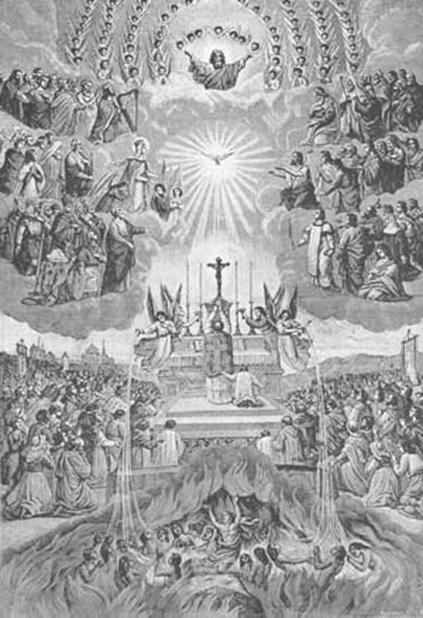
\includegraphics[scale=0.85]{gambar/purgatory2.jpg}
\end{center}

%\vspace{1cm}

\begin{center}
{\PTsmaller {Kasih, kerendahan hati, dan menurut pada kehendak Allah }}
\end{center}

\setlength{\parindent}{1cm}
\pagestyle{plain}
\chap{Apa yang harus kuketahui tentang Liturgi?} 

\section*{Pendahuluan}

Saya pernah mendengar bahwa ada orang-orang yang mengatakan liturgi di Gereja Katolik itu ‘membosankan’. Katanya lagu-lagunya itu-itu saja, kurang bersemangat dan kurang berkesan. Apa iya, demikian halnya? Sebelum berkomentar, mari kita lihat dulu apa sebenarnya arti liturgi di dalam Gereja Katolik. Lalu, setelah itu baru kita tilik kembali komentar itu. Sebab, jangan-jangan masalahnya bukan pada liturgi-nya tetapi pada diri si penerima. Ibaratnya, “kesalahan bukan pada stasiun pemancar radio, tetapi pada antena Anda.” Walaupun demikian, mari kita lihat juga apa yang perlu kita lakukan supaya kita dapat menghayati liturgi dan menjadikannya bagian dari diri kita, supaya kita tidak sampai bosan. Ini adalah bentuk “perbaikan antena” sehingga radio kita dapat menangkap sinyal dengan lebih baik.

\section*{Pengertian liturgi}

Telah kita ketahui bahwa sakramen adalah penghadiran Misteri Kristus (lihat artikel: Sakramen: Apa pentingnya dalam kehidupan iman kita?). Di dalam liturgi, Gereja merayakan Misteri Paskah Kristus yaitu sengsara, wafat, kebangkitan dan kenaikan Yesus ke surga- yang membawa kita kepada Keselamatan. Dengan merayakan Misteri Kristus ini, kita memperingati dan merayakan bagaimana Allah Bapa telah memenuhi janji dan menyingkapkan rencana keselamatan-Nya dengan menyerahkan Yesus Putera-Nya oleh kuasa Roh Kudus untuk menyelamatkan dunia. Jadi sumber dan tujuan liturgi adalah Allah sendiri.

Liturgi pada awalnya berarti “karya publik”. Dalam sejarah perkembangan Gereja, liturgi diartikan sebagai keikutsertaan umat dalam karya keselamatan Allah. Di dalam liturgi, Kristus melanjutkan karya Keselamatan di dalam, dengan dan melalui Gereja-Nya. Pada jaman Gereja awal seperti dijabarkan di dalam surat rasul Paulus, para pengikut Kristus beribadah bersama di dalam liturgi (dikatakan sebagai “korban dan ibadah iman” di dalam Flp 2:17). Termasuk di sini adalah pewartaan Injil “(Rom 15:16); dan pelayanan kasih (2 Kor 9:12). Maka, dalam Perjanjian Baru, kata ‘liturgi’ mencakup tiga hal, yaitu ibadat, pewartaan dan pelayanan kasih yang merupakan partisipasi Gereja dalam meneruskan tugas Kristus sebagai Imam, Nabi dan Raja.

Secara khusus, liturgi merupakan wujud pelaksanaan tugas Kristus sebagai Imam Agung. Dalam hal ini, liturgi merupakan penyembahan Kristus kepada Allah Bapa, namun dalam melakukan penyembahan ini, Kristus melibatkan TubuhNya, yaitu Gereja; sehingga liturgi merupakan karya bersama antara Kristus (Sang Kepala) dan Gereja (Tubuh Kristus). Konsili Vatikan II mengajarkan pengertian tentang liturgi sebagai berikut:

“Maka, benarlah bahwa liturgi dipandang sebagai pelaksanaan tugas imamat Yesus Kristus. Di dalam liturgi, dengan tanda-tanda lahiriah,  pengudusan manusia dilambangkan dan dihasilkan dengan cara yang layak bagi masing-masing tanda ini; di dalam Liturgi, seluruh ibadat publik dilaksanakan oleh Tubuh Mistik Yesus Kristus, yakni Kepala beserta para anggota-Nya.
Oleh karena itu setiap perayaan liturgis sebagai karya Kristus sang Imam serta Tubuh-Nya yakni Gereja, merupakan kegiatan suci yang sangat istimewa. Tidak ada tindakan Gereja lainnya yang menandingi daya dampaknya dengan dasar yang sama serta dalam tingkatan yang sama.”

Oleh karena itu tidak ada kegiatan Gereja yang lebih tinggi nilainya daripada liturgi karena di dalam liturgi terwujudlah persatuan yang begitu erat antara Kristus dengan Gereja sebagai ‘Mempelai’-Nya dan Tubuh-Nya sendiri.

Paus Pius XII dalam surat ensikliknya tentang Liturgi Suci, Mediator Dei, menjabarkankan definisi liturgi sebagai berikut:

\begin{quote}
\emph{“Liturgi adalah ibadat publik yang dilakukan oleh Penebus kita sebagai Kepala Gereja kepada Allah Bapa dan juga ibadat yang dilakukan oleh komunitas umat beriman kepada Pendirinya [Kristus], dan melalui Dia kepada Bapa. Singkatnya, liturgi adalah ibadat penyembahan yang dilaksanakan oleh Tubuh Mistik Kristus secara keseluruhan, yaitu Kepala dan anggota-anggotanya.”}
\end{quote}

Atau, dengan kata lain, definisi liturgi adalah seperti yang dirumuskan oleh Rm. Emanuel Martasudjita, Pr. dalam bukunya Liturgi, yaitu: “\textit{Liturgi adalah perayaan misteri karya keselamatan Allah di dalam Kristus, yang dilaksanakan oleh Yesus Kristus, Sang Imam Agung, bersama Gereja-Nya di dalam ikatan Roh Kudus.}”
Allah Bapa: Sumber dan Tujuan Liturgi

Alkitab mengatakan, “Terpujilah Allah Bapa Tuhan kita Yesus Kristus yang dalam Kristus telah mengaruniakan kepada kita segala berkat rohani di dalam sorga. Sebab di dalam Dia Allah telah memilih kita sebelum dunia dijadikan, supaya kita kudus dan tak bercacat di hadapan-Nya. Dalam kasih Ia telah menentukan kita dari semula oleh Yesus Kristus untuk menjadi anak-anak-Nya sesuai dengan kerelaan kehendak-Nya supaya terpujilah kasih karunia-Nya yang mulia, yang dikaruniakan-Nya kepada kita di dalam Dia yang dikasihi-Nya” (Ef 1:3-6). Dari sini kita mengetahui bahwa Allah Bapalah yang memberikan rahmat sorgawi kepada kita, melalui Kristus dan di dalam Kristus. Dan karena rahmat itu diberikan di dalam sakramen melalui liturgi, maka sumber liturgi adalah Allah Bapa, dan tujuan liturgi adalah kemuliaan Allah.

\section*{Kristus Bekerja di dalam Liturgi}

Karena Kristus telah bangkit mengalahkan maut, maka, Ia yang telah duduk di sisi kanan Allah Bapa, pada saat yang sama dapat terus mencurahkan Roh Kudus-Nya kepada Tubuh-Nya, yaitu Gereja-Nya, melalui sakramen-sakramen. Karena Yesus sendiri yang bertindak dengan kuasa Roh Kudus-Nya, maka kita tidak perlu meragukan efeknya, karena pasti Kristus mencapai maksud-Nya.

Puncak karya Kristus adalah Misteri Paska-Nya, maka Misteri Paska inilah yang dihadirkan di dalam liturgi Gereja. Jadi Misteri Paska yang sungguh-sungguh telah terjadi di masa lampau dihadirkan kembali oleh kuasa Roh Kudus. Karena Kristus telah menang atas kuasa dosa dan maut, maka Misteri Paska-Nya tidak berlalu begitu saja ditelan waktu, namun dapat dihadirkan kembali oleh kuasa Ilahi, yang mengatasi segala tempat dan waktu. Hal ini dilakukan Allah karena besar kasih-Nya kepada kita, sehingga kita yang tidak hidup pada masa Yesus hidup di dunia dapat pula mengambil bagian di dalam kejadian Misteri Paska Kristus dan menerima buah penebusan-Nya.

Kristus selalu hadir di dalam Gereja, terutama di dalam perayaan liturgi. Pada perayaan Ekaristi/ Misa kudus, Kristus tidak hanya hadir di dalam diri imam-Nya, namun juga di dalam wujud hosti kudus (lihat artikel: Sudahkah kita pahami arti Ekaristi?). Liturgi di dunia menjadi gambaran liturgi surgawi di mana Yesus duduk di sisi kanan Allah Bapa, dan kita semua sebagai anggota Gereja memuliakan Allah bersama seluruh isi surga.

\section*{Roh Kudus dan Gereja di dalam Liturgi}

Jika Roh Kudus bekerja di dalam diri seseorang, maka Ia akan menggerakkan hati orang tersebut untuk bekerjasama dengan Allah. Kita dapat melihat hal ini pada teladan Bunda Maria dan para Rasul. Demikian halnya liturgi menjadi hasil kerjasama Roh Kudus dengan kita sebagai anggota Gereja. Kerjasama Roh Kudus dan Gereja ini menghadirkan Kristus dan karya keselamatan-Nya di dalam liturgi, sehingga liturgi bukan sekedar ‘kenangan’ akan Misteri Kristus, melainkan adalah kehadiran Misteri Kristus yang satu-satunya itu.

Peran Roh Kudus dinyatakan pada saat pembacaan Sabda Allah, karena Roh Kudus menjadikan Sabda itu dapat diterima dan dilaksanakan di dalam hidup umat. Kemudian Roh Kudus memberikan pengertian rohani terhadap Sabda Tuhan itu, yang menghidupkan perkataan doa, tindakan dan tanda-tanda lahiriah yang dipergunakan dalam liturgi, dan dengan demikian Roh Kudus menghidupkan hubungan antara umat (beserta para imam) dengan Kristus. Selanjutnya peran Roh Kudus nyata saat konsekrasi, yaitu saat roti dan anggur diubah menjadi Tubuh dan Darah Kristus. Di sinilah puncak perayaan Ekaristi terjadi, saat Kristus berkenan menghadirkan Diri di tengah Gereja-Nya.

Oleh karena itu Sang Pelaku yang utama dalam liturgi adalah Kristus, dan kita sebagai anggota Gereja mengambil bagian di dalam karya keselamatan Allah yang dilakukan oleh Kristus itu. Dengan demikian bukan kita pribadi yang dapat menentukan segala sesuatunya dalam liturgi menurut kehendak sendiri, melainkan kita sepantasnya mengikuti apa yang telah ditetapkan oleh Tuhan Yesus dalam perayaan tersebut, sebagaimana yang telah dilakukan oleh para rasul dan diteruskan dengan setia oleh para penerus mereka.

\section*{Kristus mengajak kita ikut serta mengambil bagian dalam Misteri Keselamatan-Nya}

Yesus mengajak kita semua ikut mengambil bagian dalam karya keselamatan-Nya, terutama dalam Misteri Paska-Nya yang dihadirkan kembali di dalam Liturgi. Karena kuasa kasih dan kebangkitan-Nya, Kristus memberikan kita kesempatan yang sama dengan orang-orang yang hidup pada zaman Ia hidup di dunia 2000 tahun yang lalu, yaitu menyaksikan dan ikut mengambil bagian dalam peristiwa yang mendatangkan keselamatan kita, yaitu wafatNya di salib, kebangkitan-Nya dan kenaikan-Nya ke surga. Secara khusus penghadiran Misteri Paska ini nyata dalam Ekaristi, yang merupakan penghadiran kurban Kristus yang sama dan satu-satunya itu oleh kuasa Roh Kudus. Kuasa Roh Kudus yang dulu menghadirkan Yesus dalam rahim Maria, kini hadir untuk menghadirkan Yesus di altar. Kuasa Roh Kudus yang dulu hadir pada hari Pentakosta kini hadir di dalam setiap perayaan Ekaristi, untuk mengubah kita menjadi seperti para rasul, dipenuhi kasih dan semangat yang berkobar untuk ikut serta melakukan pekerjaan-pekerjaan Allah di dunia ini.

Jika kita menghayati kebenaran ini, kita seharusnya tidak bosan dan mengantuk dalam mengikuti misa. Sebab jika demikian, kita seumpama mereka yang hidup di jaman Yesus, hadir di bawah kaki salib Yesus, tetapi malah melamun dan tidak mempunyai perhatian akan apa yang sedang terjadi di hadapan mata mereka. Sungguh tragis, bukan? Memang Misteri Paska itu tidak hadir persis secara fisik seperti 2000 tahun lalu, namun secara rohani, Misteri Kristus yang sama dan satu-satunya itu hadir dan membawa efek yang sama seperti pada 2000 tahun yang lalu. Betapa dalamnya makna dari misteri ini, namun kita perlu menilik ke dalam hati kita yang terdalam untuk melihatnya dengan mata rohani dan menghayatinya dengan sikap tunduk dan kagum.

\section*{Bagaimana sikap kita di dalam liturgi}

Bayangkan jika Anda secara pribadi diundang pesta oleh Bapak Presiden. Tentu Anda akan mempersiapkan diri sebaik-baiknya bukan? Anda akan berpakaian yang sopan, bersikap yang pantas, mempersiapkan apa yang akan Anda bicarakan, dan Anda akan datang tidak terlambat, jika perlu siap sebelum waktunya. Mari kita memeriksa diri, sudahkah kita bersikap demikian di dalam ‘pertemuan’ kita dengan Tuhan di dalam liturgi. Karena Tuhan jauh lebih mulia dan lebih penting daripada Bapak Presiden, seharusnya persiapan kita jauh lebih baik daripada persiapan bertemu dengan Presiden.
\\{~}\\
\begin{enumerate}[label=\textbf{Langkah \arabic*}]
\item Mempersiapkan diri sebelum mengikuti liturgi dan mengarahkan hati sewaktu mengikuti liturgi
\\{~}\\
Untuk menyadari kedalaman arti misteri ini, kita harus mempersiapkan diri dengan sungguh-sungguh sebelum mengambil bagian di dalam liturgi. Persiapan ini dapat berbentuk: membaca dan merenungkan ayat kitab suci pada hari itu, hening di sepanjang jalan menuju ke gereja, datang di gereja lebih awal, berpuasa ( 1 jam sebelum menyambut Ekaristi dan terutama berpuasa sebelum menerima sakramen Pembaptisan dan Penguatan), memeriksa batin, mengaku dosa dalam sakramen Tobat sebelum menerima Ekaristi.
\\{~}\\
Lalu, sewaktu mengikuti liturgi, kitapun harus senantiasa mengarahkan sikap hati yang benar. Jika terjadi ‘pelanturan’, segeralah kita kembali mengarahkan hati kepada Tuhan. Kita harus mengarahkan akal budi kita untuk menerima dengan iman bahwa Yesus sendirilah yang bekerja melalui liturgi, dan bahwa Roh KudusNya menghidupkan kata-kata doa dan teks Sabda Tuhan yang diucapkan di dalam liturgi, sehingga menguduskan tanda-tanda lahiriah yang dipergunakan di dalam liturgi untuk mendatangkan rahmat Tuhan.
\\{~}\\
Sikap hati ini dapat diwujudkan pula dengan berpakaian yang sopan, tidak ‘ngobrol’ pada saat mengikuti liturgi, dan tidak menyalakan hp/ mengangkat telpon di gereja. Sebab jika demikian dapat dipastikan bahwa hati kita tidak sepenuhnya terarah pada Tuhan.
\\{~}\\
\item Bersikap aktif: jangan hanya menerima tetapi juga memberi kepada Tuhan
\\{~}\\
St. Thomas Aquinas mengajarkan bahwa penyembahan yang sempurna itu mencakup dua hal, yaitu menerima dan memberikan berkat-berkat ilahi. Di dalam liturgi, penyembahan kita kepada Tuhan mencapai puncaknya, saat kita kita turut memberikan/ mempersembahkan diri kita kepada Tuhan dan pada saat kita menerima buah dari penebusan Kristus melalui Misteri Paska-Nya. Puncak liturgi adalah Ekaristi, di mana di dalam Misteri Paska yang dihadirkan kembali itu, Kristus menjadi Imam Agung, dan sekaligus Kurban penebus dosa.\\{~}\\
Dalam liturgi Ekaristi, kita sebagai anggota Tubuh Kristus seharusnya tidak hanya ‘menonton’ atau sekedar menerima, tetapi ikut mengambil bagian dalam peran Kristus sebagai Imam Agung dan Kurban tersebut. Caranya adalah dengan turut mempersembahkan diri kita, beserta segala ucapan syukur, suka duka, pergumulan, dan pengharapan, untuk kita persatukan dengan kurban Kristus. Setiap kali menghadiri misa, kita bawa segala kurban persembahan diri kita untuk diangkat ke hadirat Tuhan, terutama pada saat konsekrasi, yaitu saat kurban roti dan anggur diubah menjadi Tubuh dan Darah Yesus. Dengan demikian kurban kita akan menjadi satu dengan kurban Yesus. Oleh karena itu, liturgi menjadi penyembahan yang sempurna karena Kristus yang adalah satu-satunya Imam Agung dan Kurban yang sempurna, menyempurnakan segala penyembahan kita. Bersama Yesus di dalam liturgi kita akan sungguh dapat menyembah Allah Bapa di dalam roh dan kebenaran (Yoh 4:24), karena di dalam liturgi kuasa Roh Kudus bekerja menghadirkan Kristus yang adalah Kebenaran itu sendiri.
\\{~}\\
Hal kehadiran Yesus tidak hanya terjadi dalam Ekaristi, tetapi juga di dalam liturgi yang lain, yaitu Pembaptisan, Penguatan, Pengakuan Dosa, Perkawinan, Tahbisan suci, dan Pengurapan orang sakit. Dalam liturgi tersebut, kita harus berusaha untuk aktif berpartisipasi agar dapat sungguh menghayati maknanya. Partisipasi aktif ini bukan saja dari segi ikut menyanyi, atau membaca segala doa yang tertulis, melainkan terutama partisipasi dari segi mengangkat hati dan jiwa untuk menyembah dan memuji Tuhan, dan meresapkan segala perkataan yang diucapkan di dalam hati.
\\{~}\\
\item Jangan memusatkan perhatian pada diri sendiri tetapi pada Kristus
\\{~}\\
Jadi, agar dapat menghayati liturgi, kita harus memusatkan perhatian kita kepada Kristus, dan pada apa yang telah dilakukanNya bagi kita, yaitu: oleh kasihNya yang tak terbatas, Kristus tidak menyayangkan nyawa-Nya dan mau wafat bagi kita untuk menghapus dosa-dosa kita. Kita bayangkan Yesus sendiri yang hadir di dalam liturgi dan berbicara sendiri kepada kita. Dengan berfokus pada Kristus, kita akan memperoleh kekuatan baru, sebab segala pergumulan kita akan nampak tak sebanding dengan penderitaan-Nya. Kitapun akan dikuatkan di dalam pengharapan karena percaya bahwa Roh Kudus yang sama, yang telah membangkitkan Yesus dari kubur akan dapat pula membangkitkan kita dari pengaruh dosa dan segala kesulitan kita.
\\{~}\\
Jika kita memusatkan hati dan pikiran pada Kristus, maka kita tidak akan terlalu terpengaruh jika musik atau penyanyi di gereja kurang sempurna, khotbah kurang bersemangat, kurang keakraban ataupun hawa panas dan banyak nyamuk. Walaupun tentu saja, idealnya semua hal itu sedapat mungkin diperbaiki. Kita bahkan dapat mempersembahkan kesetiaan kita disamping segala ketidak sempurnaan itu- sebagai kurban yang murni bagi Tuhan. Langkah berikutnya adalah, apa yang dapat kita lakukan untuk turut membantu memperbaiki kondisi tersebut. Inilah salah satu cara menghasilkan ‘buah’ dari penerimaan rahmat Tuhan yang kita terima melalui liturgi.
\end{enumerate}

\section*{Liturgi adalah sumber kehidupan}

Jadi sebagai karya Kristus, liturgi menjadi kegiatan Gereja di mana Kristus hadir dan membagikan rahmat-Nya, yang menjadi sumber kehidupan rohani kita. Walaupun demikian, liturgi harus didahului oleh pewartaan Injil, iman dan pertobatan, sebab tanpa ketiga hal tersebut akan sangat sulit bagi kita untuk menghayati perayaan liturgi, apalagi menghasilkan buahnya dalam kehidupan sehari-hari. Ibaratnya tak kenal maka tak sayang, maka jika kita ingin menghayati liturgi, maka sudah selayaknya kita mengetahui makna liturgi, menerimanya dengan iman dan menanggapinya dengan pertobatan.

Liturgi yang bersumber pada Allah menjadi sumber dan puncak kegiatan Gereja. Bersumber pada liturgi ini, Gereja menimba kekuatan untuk melaksanakan pembaharuan di dalam Roh, misi perutusan, dan menjaga persatuan umat. Maka jika kita mengalami ‘kemacetan ataupun percekcokan’ di dalam kegiatan paroki, petunjuk praktis untuk memeriksa adalah: Sudah cukupkah keterlibatan anggota dalam Ekaristi -tiap minggu atau jika mungkin setiap hari? Adakah kedisiplinan anggota untuk mengaku dosa di dalam Sakramen Tobat secara teratur, misalnya sebulan sekali? Walaupun demikian, kehidupan rohani kita tidak terbatas hanya dari keikutsertaan dalam liturgi, tetapi juga dari kehidupan doa yang benar (doa pribadi (Mat 6:6) dan doa tanpa henti (1Tes 5:17)).

\section*{Kesimpulan}

Seperti telah diuraikan di atas: liturgi merupakan partisipasi kita di dalam doa Kristus kepada Allah Bapa oleh kuasa Roh Kudus. Liturgi terutama Ekaristi yang menghadirkan Misteri Paska Kristus merupakan peringatan akan karya Allah Tritunggal untuk mendatangkan keselamatan bagi dunia. Maka liturgi merupakan puncak kegiatan Gereja, dan sumber di mana kuasa Gereja dicurahkan, yaitu kehidupan baru di dalam Roh, keikutsertaan di dalam misi perutusan Gereja dan pelayanan terhadap kesatuan Gereja. Jadi bagi kita umat beriman, terutama yang ikut ambil bagian di dalam karya kerasulan awam, keikutsertaan di dalam liturgi merupakan sesuatu yang utama. Tidak bisa kita melayani umat, jika kita sendiri tidak diisi dan diperbaharui oleh rahmat Tuhan sendiri. Prinsipnya, “kita tidak bisa memberi, jika kita tidak terlebih dahulu menerima” rahmat yang dari Allah.

Rahmat Allah ini secara nyata kita terima melalui liturgi. Dalam hal ini, Ekaristi memegang peranan penting karena di dalamnya rahmat yang diberikan adalah Kristus sendiri. Kini tinggal giliran kita untuk memeriksa diri dan mempersiapkan hati untuk menerima berkat rahmat itu. Jika kita mempunyai sikap hati yang benar dan berpartisipasi aktif di dalam liturgi, maka Tuhan sendiri akan memberkati dan menjadikan kita anggota TubuhNya yang menghasilkan buah bagi kemuliaan nama-Nya. Menimba bekal rohani melalui liturgi merupakan salah satu cara yang paling nyata untuk menjawab undangan Tuhan Yesus, “Tinggallah di dalam Aku dan Aku di dalam kamu…. Barang siapa tinggal di dalam Aku dan Aku di dalam dia, ia berbuah banyak, sebab di luar Aku kamu tidak dapat berbuat apa-apa” (Yoh 15:4-5).

\vfill
\noindent{\framebox{\parbox{10cm}{\centering\emph{
 ``Allah itu pengada sempurna yang tak terbatas,
 yaitu Tritunggal''\\
 (Santo Turibus dari Montenegro)
}}}}

%\chap{Orang Muda Katolik (OMK) dan Liturgi}

\section*{Prasangka}
\small
Dalam praktek, banyak kali muncul masalah pada relasi antara OMK dan liturgi (perayaan iman, ibadat). Di antara liturgi dan OMK seolah ada hubungan ”enggan tapi rindu”. Di balik tema “liturgi dan orang muda”, masih bercokol  prasangka laten baik terhadap Orang Muda Katolik (OMK), maupun terhadap Liturgi Gereja Katolik Roma. OMK seolah-olah suka hura-hura, semaunya sendiri, tidak bisa diatur dalam berliturgi. Sebaliknya, liturgi sering dipandang sebagai aturan sakral dan baku, seakan-akan jauh dari gelora kerinduan orang muda. Terhadap OMK, Tim Liturgi Paroki biasanya mengenakan frasa ”OMK yang pragmatis, maunya serba lain”. Seakan-akan OMK diperlawankan dengan liturgi yang tak memberi ruang kebebasan ungkapan iman. Dari pihak OMK, ada pula prasangka, bahwa liturgi itu serba  kaku.

Prasangka ini  bisa dipahami, karena sifat umum orang muda yang masih dalam masa pertumbuhan yang pesat. Mereka sedang berkembang dalam dimensi psikologis, intelektual, seksual-hormonal, emosi, peran sosial dan iman. OMK memang sedang  mengalami transformasi menuju kepribadian yang integral. Rentang masa muda yang panjang (usia 13-35 th) adalah masa distingtif,  saat mencari, mempertanyakan, belajar dan mengambil keputusan. Kita yang pernah menjalani masa muda tentu merasakan bahwa saat itu merupakan saat yang sukar, menantang sekaligus menggairahkan karena penemuan-penemuan baru. Sering kali kita ingin sesuatu yang ”lain dari pada yang lain” pada masa muda. Sedangkan di pihak lain, Liturgi Gereja Katolik Roma, sudah berkembang dalam 20 abad dan sering dipandang sebagai peraturan yang kaku alih-alih sebagai perayaan yang membebaskan. Padahal, potret berliturgi oleh OMK tak selamanya demikian.

Prasangka dan kecurigaan  yang digeneralisasi begitu saja terhadap OMK itu tentu tidak akan memecahkan persoalan yang sering kali muncul dalam praktek penghayatan OMK terhadap liturgi. Tidak bijaksana,  generalisasi mengenai OMK yang ”pragmatis dan maunya serba lain” itu. Liturgi Gereja pun tidak sepantasnya diperlawankan dengan gejolak dan selera orang muda. Kenyataannya, bahwa banyak orang terpanggil menjadi kudus pada masa muda, dan panggilan kekudusan itu banyak yang bermula dari penghayatan liturgi. Kita pun tahu, Ekaristi Kaum Muda (EKM) baik yang diselenggarakan oleh paroki, maupun oleh Panitia \textit{World Youth Day} yang mendatangkan Sri Paus sebagai pemimpin liturgi, selalu dipenuhi OMK dengan kerinduan mendalam. Bahkan, kelompok misa bahasa Latin yang terkesan ”penuh aturan ketat” ada yang digerakkan  oleh orang muda.

\section*{Memerlukan Dukungan}

Seperti pada umumnya orang Katolik Indonesia, tua maupun muda, penghayatan OMK akan liturgi sebenarnya tergantung pada pengetahuan dan pengalaman mereka akan liturgi itu sendiri. Bahwa praktek liturgi OMK kadang-kadang membuat para penanggungjawab liturgi mengerutkan kening, bagi saya lumrah saja dalam konteks pembelajaran. Gelegak kreativitas masa muda sekaligus tingkat pengetahuan dan pengalaman OMK akan liturgi haruslah bisa dipahami dan didukung. Tak usahlah daya kreatif mereka dalam ber-liturgi dihakimi dengan sewenang-wenang seperti yang sering terdengar dari keluhan mereka. Gara-gara  maunya kreatif, mereka ”dikecam secara liturgis”.

Sepanjang pengalaman para pendamping, tak ada OMK yang menjadi buruk karena mau kreatif dalam merencanakan dan mengolah liturgi. Justeru sebaliknya, para aktivis kelompok-kelompok OMK yang mau proaktif , mau belajar, mau secara jujur mengusulkan berbagai kreasi dalam liturgi, dan karenanya  berani mencari dan melakukan yang benar, berani mengakui  kesalahan bila terjadi dan berani memperbaikinya) terbukti menjadi aktivis  dengan penghayatan liturgi yang nyata dalam perilaku. Lagipula, jika OMK membuat kesalahan dalam ber-liturgi, ternyata kesalahan itu tidaklah fatal, normal saja. Kesalahan mereka pun kadang-kadang karena pengaruh kelompok kategorial  yang lebih senior. Justeru kelompok-kelompok kategorial yang beranggotakan orang-orang tidak muda lagi lah yang sering bikin kesalahan fatal, dan keras kepala, bukan? Sebaliknya, biasanya dengan taat OMK mau belajar dari kesalahan. Mereka tetap gembira dan kreatif, asalkan pendamping dengan empati mau  setia mendampingi, menjelaskan makna simbol dan hakikat liturgi yang kaya makna itu kepada mereka, memetakan posisi kelompok dalam lebensrauung Gereja lokal, dsb. Saya yakin, dalam kerja sama yang baik dengan pendamping itu dapatlah dihindarkan kesalahan-kesalahan fatal yang tidak perlu terjadi. Sebenarnyalah di antara Liturgi dan OMK ada hubungan batin yang saling mendukung. Liturgi menjadi ongoing formation  bagi OMK. Sedangkan daya kreativitas dan gelora kemudaan OMK membuat liturgi dirayakan dengan bersemangat. Liturgi tanpa keterlibatan orang muda, merupakan tanda nyata kematian Gereja.
\normalsize

\section*{Liturgi Kelompok OMK}

Ketika naskah ini diketik (Mei 2008-pen), kantor Youth Desk – FABC di Manila sedang mengolah survei mengenai penghayatan OMK akan Liturgi Ekaristi. Munculnya jajak pendapat untuk OMK mengenai Ekaristi ini didasari praduga bahwa kerinduan OMK akan liturgi berbanding lurus dengan pengetahuan dan pengalaman mereka ber-liturgi.  Tema Liturgi Ekaristi menjadi pembahasan dalam \textit{Asian Youth Day} tahun  2009 di Manila.  Mengapa tema ini diagendakan? Saya menduga, di satu sisi ada kecemasan kalau-kalau  Liturgi  ”ditinggalkan” alias ”tidak laku” lagi di kalangan OMK. Liturgi disangka tidak mampu menjawab kerinduan OMK di tengah arus percepatan globalisasi yang mengasingkan OMK. Di sisi lain ada pula kecemasan kalau-kalau  OMK di berbagai kelompok kategorial yang masih mau aktif ber-liturgi  mulai ”meninggalkan” kaidah liturgi, alias ”mengikuti maunya sendiri”. Komunitas-Komunitas OMK  lebih mementingkan ”rasa kepuasan kelompok” dalam berliturgi dibandingkan ”rasa universal” Gereja. Dua macam kecemasan itu bermuara pada dua pertanyaan atas satu kenyataan liturgi: 
\begin{enumerate}
\item Bagaimanakah liturgi menjawab kerinduan OMK akan perasaan ditemani oleh ”Yang Ilahi” di tengah arus zaman dan perubahan selera ini? \item Bagaimanakan OMK menyadari tanggungjawab dan penghayatannya akan liturgi yang bergairah karena setia pada aturan Gereja?
\end{enumerate}

Saya menemukan dua prasyarat atas jawaban pertanyaan di atas setelah mengamati beberapa komunitas OMK.  Prasyarat itu adalah 
\begin{enumerate}
\item Jika mereka mendapatkan komunitas yang digembalakan dengan semangat berbagi dan mereka dipercaya dalam kegiatan komunitas. 
\item Jika ungkapan kemudaan mereka diberi ruang dan waktu yang cukup dalam liturgi komunitas.
\end{enumerate}

Pada beberapa kelompok OMK, liturgi mereka hayati sepenuh hati. Tampaknya mereka ”puas” dan selalu rindu dengan liturgi komunitas mereka.  Sebabnya, liturgi tak mereka lepaskan  dari kehidupan komunitas kategorial mereka, dan bahwa komunitas memberi ruang dan waktu bagi karakter kemudaan mereka dalam liturgi. Ada ”gembala” (pendamping/ moderator) yang secara tetap mempercayai mereka dalam kegiatan komunitas. Sang pendamping ini (imam dan biarawati/awam) mendampingi liturgi mereka dengan tak bosan mengajarkan prinsip-prinsip  liturgi  sesuai  maksud Gereja. Beberapa kelompok OMK itu adalah: Komunitas Sant’ Egidio (SE), beberapa komunitas Persekutuan Doa Karismatik Katolik (PDKK) muda-mudi, beberapa sel Komunitas  Tritunggal Mahakudus (KTM) muda-mudi; beberapa presidium Legio Mariae (LM) muda-mudi, kelompok Imago Dei (ID), dan kelompok Doa Taize (DT). Mereka memiliki kesamaan pengalaman, bahwa perjumpaan dengan Allah dalam doa, teristimewa liturgi merupakan puncak dan sumber spiritualitas dan kegiatan komunitas.

\section*{Variasi yang Melegakan}

Kelompok-Kelompok OMK itu  biasa berkumpul untuk berdoa secara rutin.  Pertemuan doa mereka mengikuti bukanlah liturgi karena dan karenanya memiliki variasinya masing-masing.  Dalam hal ini Tata Perayaan Sabda atau Ibadat Sabda atau Doa kelompok kategorial di luar Ekaristi, adalah kegiatan non liturgis atau para liturgi atau devosi. Perayaan Sabda adalah liturgi bila dilakukan dalam Ibadat Harian dan liturgi sakramen termasuk Ekaristi yang meliputi dua bagian utama: liturgi Sabda dan Liturgi Ekaristi. Ibadat Sabda di luar liturgi atau para liturgi dan devosi tidak sangat terikat pada kaidah-kaidah liturgi. Dalam hal ini kreativitas orang muda mendapat ruang yang lebih luas dan nyaman. Sebulan atau beberapa bulan sekali mereka mengundang imam untuk merayakan ekaristi. Umumnya, mereka mengikuti aturan liturgi yang baku. KTM dan PDKK  secara berkala membuat adorasi sakramen Mahakudus. Sebaiknya Adorasi Sakramen Mahakudus dibuat sebelum atau sesudah Perayaan Ekaristi, atau sebagai unsur dari Ritus Penutup Ekaristi, dan bukan di tengah liturgi Sabda atau di tengah liturgi Ekaristi.  Beberapa variasi liturgi, khususnya dalam perayaan ekaristi dan adorasi, tampak paling ekstensif dalam PDKK dan KTM.

Lagu-lagu yang dipakai KTM dan PDKK sebagian besar bercorak mirip pop rohani. Ciri khas liturgi PDKK dan KTM adalah sangat ekspresif. Bernyanyi melambungkan pujian kepada Allah, sambil bertepuk tangan, mengangkat tangan, diiringi musik yang meriah. Di sini dikenal juga pencurahan Roh. Salah satu yang khas pula dalam PDKK dan KTM ialah peran pemimpin doa yang mengantar sesi-sesi lagu, doa dan firman. Dalam perayaan ekaristi, ada kesan bahwa peran imam  sebagai pemimpin resmi liturgi Gereja, tenggelam oleh peran pembawa acara yang juga pemimpin doa. Ambil contoh, pengantar tobat yang dibawakan imam, sering kali masih diulang oleh pemimpin doa dengan lebih panjang. Bagaimana hal ini menjadi variasi yang tidak mengganggu? Kuncinya, dialog persiapan antara imam dan pemimpin doa.  Menjadi soal jika imam tidak diajak bicara dahulu  dan celakanya merasa tidak rela karena dilangkahi dalam memimpin doa. Bisa jadi saat homili menjadi saat pelampiasan ketidakpuasan imam. Namun hal ini jarang sekali terjadi dalam kelompok doa OMK. Pemimpin doa komunitas PDKK dan KTM OMK biasanya bisa bekerja sama dengan baik dengan imam pemimpin ekaristi.

Pertemuan doa  DT mendaraskan mazmur dan doa singkat dalam nada sederhana dengan musik lembut dan dekorasi temaram dengan ikon salib Kristus di altar depan. Doa-doa  Sant’ Egidio mirip dengan DT. ”Mereka biasa berdoa sebentar di depan ikon Yesus. Ini sungguh doa inklusif. Pemimpinnya tidak menempatkan diri di depan umat (di belakang altar), tetapi di depan umat. Kalau ada imam ingin berbagi atau memberi keterangan Sabda Tuhan, barulah beliau tampil di mimbar. Hal ini wajar karena pertemuan doa mereka ini bukanlah perayaan Ekaristi.  Sejauh perlu, doa dilakukan “bersama” di depan ikon Yesus. Doa ini juga merupakan relativisasi di hadirat Tuhan. Orang, setelah seharian bekerja, tidak mensyukuri prestasinya atau mengumpat kegagalan hari itu, melainkan mempersembahkan seluruh perjuangan sepanjang hari kepada Tuhan, entah sukses, entah gagal, entah biasa-biasa saja. Sebetulnya cara pandang seperti ini biasa saja. Hanya saja, doa ini dikemas dalam suatu liturgi yang menyentuh hati: di depan ikon besar Yesus, dalam keredupan cahaya gereja, dengan koor satu suara, sederhana, dengan iringan organ, tapi mengantar pada keagungan Tuhan. Liturgi mereka tidak ada yang istimewa. Pengalaman mereka yang selalu dibawa dalam doa-doa harian dan misa di akhir pekan, itulah yang istimewa.

ID mengungkapkan doa bersama sebagai sarana berkomunikasi dengan Tuhan, untuk mengetahui kehendak-Nya, mendapatkan restu, serta mendapat kekuatan. Dasar kegiatan ID ialah saling menguatkan dalam doa (Gal. 6:2; Ef. 6:18-20). Suasana praise and  worship bersifat fun, gembira penuh syukur. Namun jika dilakukan dalam Liturgi (misalnya Ekaristi), apapun bentuk variasi penyesuaian, hendaknya tidak timbul kesan bahwa di tengah liturgi dimasukkkan acara gembira ria yang bersifat profan.  Mereka pun mencari \textit{rhema} untuk minggu itu dan mengungkapkan dalam liturgi.

LM menempatkan devosi kepada Bunda Maria. Namun yang menjadi sentralnya ialah Allah Bapa, Putra dan Roh Kudus.  Semua pusat devosi, ibadat, liturgi adalah Allah: Bapa, Putra dan Roh Kudus. Maka devosi yang khusus kepada Maria itu tidak harus mengaburkan atau menghilangkan sentralnya, tetapi justru semakin mengarahkan para devosan ke sentral: \textit{ad Iesum, ad Patrem, ad Spiritum Sanctum}, itu sebabnya semua orang yang berdoa rosario atau mempunyai devosi khusus kepada Bunda Maria menyalaminya sebagai Putri Allah Bapa, Bunda Allah Putra dan Mempelai Allah Roh Kudus. \textit{Per Mariam ad Iesum}.  Doa  mereka mengikuti tatacara dalam Buku Pegangan LM. Lagu sangat minim, kalaupun ada,  lagu penghormatan kepada Bunda Maria selalu dinyanyikan dengan khusuk. Kerendahan hati dan kesederhanaan menjadi pola doa  kelompok ini. Doa rosario dan \textit{catena legionis} diwajibkan dalam devosi mereka. Jika ada misa, doa rosario dan catena legionis wajib didoakan tetapi sebelum liturgi, sebelum Ekaristi, yang berarti di luar liturgi dan bukan di tengah liturgi. Ini sangat tepat, walaupun mungkin ada yang kurang paham lalu mendoakannya dalam liturgi. Tak banyak OMK yang terlibat dalam LM dibanding kelompok lain.

Walaupun berbeda ungkapan, namun nyatalah bahwa perasaan mereka sama-sama terangkat kepada kehadiran Yang Ilahi dan iman dimantapkan. Adanya penyesuaian dan variasi itu dirasakan melegakan  OMK dalam menghayati iman akan Allah.

\section*{Liturgi yang Tergairahkan oleh Kemudaan}

Apakah istimewanya liturgi orang muda? Sebenarnya tatacara liturgi mereka tidak ada bedanya dengan liturgi pada umunya. Yang istimewa adalah apa yang mereka rindukan dan  cara ungkapannya. Dalam situasi pertumbuhan menuju masa depan yang tidak serba jelas, di tengah zaman yang hiruk pikuk tidak pasti, liturgi menjadi wahana ungkapan mereka. Apakah liturgi bisa menjawab kerinduan mereka? Alih-alih menunggu liturgi memuaskan mereka, maka banyak kali terjadi, mereka-lah yang berinisiatif menggairahkan liturgi sesuai desakan kuat di dalam dada untuk mengungkapkan kerinduan mereka akan Allah. Sayangnya, para penanggungjawab liturgi kadang-kadang tidak (mau) menanggapi dengan sabar. Akibatnya, gairah OMK sering dikecewakan. Yang diperlukan sekarang adalah penanggungjawab liturgi yang melibatkan OMK dalam tim liturgi, agar perencanaan doa-doa dan lagu, serta variasi lain bisa menjawab kerinduan OMK. Ada aneka warna kelompok doa OMK. Sangat bagus jika mereka dilibatkan oleh para penanggungjawab liturgi di berbagai tingkat (paroki, dekenat/kevikepan, dan keuskupan) untuk menggairahkan liturgi kita. Dengan demikian, tak kan ada lagi kecurigaan dan penilaian sepihak atas OMK seperi pada alinea pertama tulisan ini. Mereka pun merasa tersapa dan pasti belajar liturgi Katolik dengan lebih baik. Ada satu lagi potret ber-liturgi OMK walaupun sangat jarang. Yakni OMK yang tergerakkan oleh liturgi sedemikian rupa, sehingga terinspirasi untuk terjun dalam perjuangan menegakkan perdamaian dan keadilan. Mereka pun perlu dilibatkan dalam perencanaan dan pelaksanaan liturgi agar liturgi benar-benar ”puncak dan sumber” hidup beriman bagi OMK.

\section*{OMK dan Musik Liturgi}

Bayangkanlah suatu perayaan Liturgi Ekaristi di gedung gereja yang besar dengan ribuan OMK. Bagaimana jika tanpa musik? Nah, musik ialah salah satu kegemaran favorit OMK, sejak era zaman batu hingga era dot com ini. Namun musik Liturgi, memiliki ketentuan liturgis. Apakah OMK masih tertarik dengan musik liturgi? Atau, apakah musik liturgi masih mampu berdaya pikat terhadap OMK?

Perayaan Liturgi  tidak melulu  pikiran (ratio) . Liturgi selalu meliputi tata gerak dan menyangkut  seluruh kekayaan cita-rasa batin yang mendorong setiap orang untuk mengungkapkannya secara lahir. Wujudnya doa, permohonan, pujian, sembah sujud, dan semacamnya. Relasi dengan Allah ialah misteri. Maka apa pun yang sulit dinyatakan dalam kata-kata, diwujudkan dalam seni yaitu musik, syair, nyanyian, lukisan, pahatan yang menembus misteri relasi Allah dan manusia. Itulah jiwa Liturgi, yaitu Allah yang selalu ingin mengkomunikasikan diri kepada manusia dan manusia yang rindu menyambut-Nya. Ungkapan itu diungkapkan oleh manusia dengan segala dimensi kemanusiaannya. Di sinilah kita tempatkan musik dan seni liturgi. Tujuan Musik Liturgi ialah kemuliaan Allah dan pengudusan manusia (Konstitusi tentang Liturgi, / \textit{Sacrosanctum Concilium}, SC, 112) dan Alkitab memuji lagu-lagu ibadat (Ef 5:19; Kol 3:16)

Yang harus diketahui ialah perbedaan antara Musik / Lagu Liturgi dan Musik / Lagu Rohani Umat.   Ketika ungkapan musik diwujudkan dalam perayaan Liturgi, maka kita mengenal istilah Musik/ Nyanyian Liturgi ; sedangkan ketika ungkapan musik diwujudkan dalam perayaan non-liturgi, maka kita mengenal istilah Nyanyian rohani umat (populer). Dalam Musik/Lagu Liturgi Ada 3 kekuatan yang terkandung sesuai hakikat perayaan Liturgi:
\begin{enumerate}
\item Dinamisme iman pribadi

\item Dinamisme misteri Allah Bapa melalui Kristus dalam Roh Kudus.

\item Dinamisme komunitas Gerejawi sebagai anggota Tubuh mistik Kristus.
\end{enumerate}

Komponen musik Liturgi adalah ungkapan komunikasi-komunal antara  saya – kita – Allah Tritunggal dalam cara yang lebih mesra dan batiniah.

Lagu/Nyanyian Rohani Umat atau Lagu Rohani Populer, tidak mengandung hakikat  tiga kekuatan dinamis terebut. Musik rohani merupakan ungkapan iman personal saja, belum eklesial/Gerejawi dan sering juga tidak memperhitungkan dimensi dinamika Allah Tritunggal. Namun SC 118 mengingatkan agar nyanyian rohani umat dikembangkan secara ahli, sehingga kaum beriman dapat bernyanyi dalam kegiatan devosional dan perayaan-perayaan ibadat menurut ketentuan rubrik.

Dalam dokumen “\textit{Musicam Sacram}” artikel 5 dikatakan sbb:

\begin{quote}
\emph{Sungguh, lewat bentuk  ini (musik-pen), doa diungkapkan secara lebih menarik, dan misteri Liturgi, yang sedari hakikatnya bersifat hirarkis dan jemaat, dinyatakan secara lebih jelas. Kesatuan hati dicapai secara lebih mendalam berkat perpaduan suara. Hati lebih mudah dibangkitkan ke arah hal-hal surgawi berkat keindahan upacara kudu \ldots”}
\end{quote}

Apabila telah dipahami betapa luhurnya misteri yang terjadi selama perayaan Liturgi maka perlulah OMK menyadari betapa luhurnya peran musik dan nyanyian dalam Liturgi sebagai sarana komunikasi dengan yang ilahi dalam kebersamaan.

\textit{Sacrosanctum Concilium} artikel 112 menyebutkan peran musik sebagai tugas pelayanan untuk mendukung ibadat kepada Allah. Paus Pius X menyebutnya sebagai umile ancella. Paus Pius XI menyebutnya sebagai \textit{serva nobilissima}. Paus Pius XII menyebutnya sebagai \textit{sacrae liturgiae quasi administra}. Dan Konsili Vatikan II menyebutnya: \textit{munus ministeriale in dominico servitio} (tugas pelayanan dalam mengabdi Tuhan).

\subsubsection*{Syarat-syarat Musik Liturgi}
\begin{enumerate}
\item    Harus merupakan musik sejati menurut seni musik.
\item    Kata-kata dan nada harus sungguh menghantar manusia kepada Allah, oleh karena itu harus berdasarkan teks Kitab Suci dan Teks Liturgi.
\item    Harus mengungkapkan daya-daya seni dan religiositas dalam dialog dan tanda-tanda simbolik lainnya selama berlangsung perayaan, di mana Allah dimuliakan dan umat beriman dikuduskan.
\end{enumerate}

Maka Musik Liturgi semakin suci, bila semakin erat hubungannya dengan upacara Ibadat, entah dengan mengungkapkan doa-doa secara lebih mengena, entah dengan memupuk kesatuan hati, entah dengan memperkaya upacara suci dengan kemeriahan yang lebih semarak. Gereja menyetujui segala bentuk kesenian yang sejati, yang memiliki sifat-sifat menurut persyaratan Liturgi, dan mengizinkan penggunaannya dalam Ibadat kepada Allah (SC 112).

\section*{Ekaristi untuk Orang Muda}

\textit{Actio Pastoralis}, instruksi Kongregasi Ibadat mengenai “Misa untuk kelompok-kelompok khusus” 15 Mei 1969 menyatakan ”Gereja sangat menganjurkan penyelenggaraan Misa untuk berbagai kelompok dalam paroki baik territorial maupun kategorial sebab mempunyai dampak lebih mendalam terhadap penghayatan hidup kristiani, saling mendukung dalam perkembangan hidup rohani dan kesaksian iman”.

Untuk itu diperlukan berbagai penyesuaian, yang dapat dibagi dalam dua kategori:
\begin{enumerate}
\item penyesuaian akomodatif
\item penyesuaian inkulturatif
\end{enumerate}

\textbf{Akomodatif}  maksudnya penyesuaian dalam hal-hal yang tidak berkaitan dengan budaya setempat misalnya: bacaan, nyanyian, cara berkomunikasi, tata-gerak ritual, dramatisasi, tarian,  dll. Misa Orang Muda perlu banyak penyesuaian sesuai dengan jiwa mereka agar sungguh berdaya-guna bagi hidup mereka, namun mengindahkan kaidah liturgi.

\textbf{Inkulturatif} maksudnya  unsur-unsur budaya setempat di mana dituntut studi yang mendalam mengenai unsur-unsur yang dapat dimanfaatkan untuk membantu kelompok-kelompok masyarakat tertentu dalam penghayatan iman mereka.

\section*{Harapan}

Semoga dengan demikian musik dan lagu liturgi menyemarakkan cita rasa batin yang terdalam dari OMK. Musik yang dipakai dalam liturgi haruslah yang menjunjung rasa hormat sembah bakti dalam memuliakan Allah, dan membuat OMK sadar dan aktif dalam liturgi.


\sumber{Yohanes Dwi Harsanto Pr\\ (Sekretaris Eksekutif komisi Kepemudaan KWI)\\
http://www.katolisitas.org} 
\chap{\textit{Sadar Liturgi}\\Memahami liturgi lewat karikatur}

Liturgi sudah sering kita dengar. Namun tidak jarang kita kurang mengerti mengenai liturgi yang sering kita ikuti di gereja. Kita mungkin pernah mendapat pemahaman tentang liturgi saat katekumen atau saat mau menerima sakramen penguatan. Mungkin juga saat pelajaran agama di sekolah. Biasanya kita mendengar penjelasan dari pengajar atau kita disodori buku atau catatan untuk dibaca. 

Namun cara yang ditempuh seorang Romo ini untuk menjelaskan masalah liturgi, menjadi agak lain. Sebagai pendamping situs http://www.imankatolik.org Romo F.X. Agis Triatmo O.Carm. menyuguhkan karyanya berupa karikatur untuk memberikan pemahaman mengenai liturgi.

Karikatur-karikatur itu berisi gambar dan dibubuhi keterangan seperlunya. Sudah ada 50 karikatur yang diselesaikan dan akan menyusul 50 karikatur lagi. Ada komentar atau gambar yang bisa membangkitkan senyum saat kita mengamatinya. Untuk versi lengkap silakan buka di http://www.imankatolik.or.id/sadar.html.

\begin{center}
\includegraphics[scale=0.8]{../sadar-liturgi/sadar_liturgi_rm_fx_agis_triatmo_OCarm_1.jpg}


\includegraphics[scale=0.8]{../sadar-liturgi/sadar_liturgi_rm_fx_agis_triatmo_OCarm_4.jpg}

\includegraphics[scale=0.8]{../sadar-liturgi/sadar_liturgi_rm_fx_agis_triatmo_OCarm_5.jpg}


\includegraphics[scale=0.8]{../sadar-liturgi/sadar_liturgi_rm_fx_agis_triatmo_OCarm_6.jpg}

\includegraphics[scale=0.8]{../sadar-liturgi/sadar_liturgi_rm_fx_agis_triatmo_OCarm_7.jpg}

\includegraphics[scale=0.5]{../sadar-liturgi/sadar_liturgi_rm_fx_agis_triatmo_OCarm_14.jpg}

\vspace{2cm}

\includegraphics[scale=0.6]{../sadar-liturgi/sadar_liturgi_rm_fx_agis_triatmo_OCarm_19.jpg}

\end{center}

\chap{\textit{Cerpen}\\Stroke sembuh: Terpujilah kristus!}
\small

	Tidak ada angin tidak ada hujan, suatu sore datang Mas Martin ke rumah saya. Nama lengkapnya Martinus Hendro Winarto. Sudah lama sekali kami tidak saling bertemu. Mungkin ada sekitar 15 tahun. Dulu sering bersama-sama nonton teater, diskusi soal sastra, jurnalistik dan kebudayaan. Tetapi kedatangannya sore itu tidak ada kaitannya dengan seni dan budaya. Ia datang minta tolong kepada saya agar mau membantu menyembuhkan ayahnya yang sedang sakit karena serangan stroke.

	“Lho, piye to \ldots kok mas Martin datang pada saya? Ya mbok ke dokter atau rumah sakit! Saya ini kan bukan paranormal atau penyembuh alternatif!” kata saya benar-benar heran.

	“Jangan merendah to, Mas Agung. Rendah hati memang bagus, tetapi jauh lebih bagus kalau kamu mau menolongku.” Kata mas Martin.

	Saya hanya menggeleng-gelengkan kepala. “Wee, lha edan tenan iki!” kata saya dalam hati. Mas Martin lalu cerita bahwa sudah tiga bulan ayahnya tidak berdaya karena stroke. Pengobatan ke dokter di rumah sakit sudah rutin dilakukan tetapi hasil kesembuhannya belum maksimal. Ayahnya masih bisa jalan pelan-pelan, namun harus dibimbing. Padahal umurnya baru 56 tahun. Untunglah, semangat hidup pak Paulus Pujo Winarto, ayahnya itu, masih tinggi. Pernah ia minta dibawa ke Sendangsono, meski harus didorong dengan kursi roda hingga di depan Bunda Maria. Sembilan kali dia dibawa ke Sendangsono dan pada ziarah yang ke Sembilan pak Paulus dimandikan dengan air sendang.

	“Tetapi belum sembuh juga. Karena itu mewakili keluarga, saya datang kemari minta pertolongan padamu.” Kata mas Martin sungguh-sungguh.

	Meski saya yakinkan berkali-kali jika saya ini tidak bisa menyembuhkan penyakit, bahkan saya ini termasuk kategori manusia tidak sehat, tetapi mas Martin tetap memaksa. “Apapun yang kamu katakan akan kami turuti. Yang penting ayah saya bisa sembuh!” begitu kata mas Martin sebelum pamit pulang. 

\section*{Bisikan Bunda}

	Siapa tidak pusing tujuh keliling jika tiba-tiba mendapat “cobaan” seperti itu? Sumpah mati saya belum pernah mempelajari metode penyembuhan model apapun. Saya sendiri termasuk orang yang sakit-sakitan. Ini buah dari hobi melamun, duduk-duduk sambil membaca dan agak alergi dengan olah raga. Lalu tiba-tiba diminta tolong untuk menyembuhkan orang sakit stroke.

	Bunda Maria, bagaimana anakmu ini? Bukan paranormal, bukan dukun, bukan akupunturis, bukan ahli prana, bukan dokter, tidak punya kesaktian, lalu harus menyembuhkan orang sakit.

	Tuhan Yesus, Engkau sering membuat mujizat. Menyembuhkan orang lumpuh, orang buta, perempuan yang pendarahan, orang kerasukan setan, bahkan menghidupkan orang mati. Engkau bisa sebab Engkau adalah Putra Allah. Lalu saya ini apa? Pendosa yang ringkih. Hamba yang tidak setia. Sahabat yang sering berkhianat.

	Santo Petrus berani berbuat seperti Diri-Mu, menyembuhkan orang lumpuh sebab dia adalah rasul-Mu, yang pernah hidup -Mu, pernah menjamah jubah-Mu, makan bersama dan duduk berdekatan dengan-Mu. Karena itu dia pasti ‘ketularan’ kesaktian-Mu.

	Semalam suntuk saya tidak bisa tidur. Esoknya dengan sepeda motor butut saya lari ke Sendangsono. Seharian penuh saya duduk didepan patung Bunda Maria. Segala kebingungan saya tumpahkan di depan Bunda Maria.

	Pukul tiga sore, antara tidur dan terjaga, saya seperti mendengar bisikan halus: \textit{Bawalah kemari. Biarkan dia berjalan sendiri.} Dalam perjalanan pulang bisikan itu terus mengiang-ngiang di telinga saya. Dan bahkan saya yakin itu bukan bisikan roh halus yang tinggal di pohon angsana dan pohon beringin di Sendangsono. Itu adalah bisikan Bunda Maria!

\section*{Mulailah berjalan sendiri}

	“Mas Agung, apa yang harus kami lakukan?” Tanya mas Martin lima hari kemudian. “katakan apa saja, asal kami sanggup melakukan, pasti kami lakukan. Yang penting ayah kami bisa sembuh!” lanjutnya serius. Ia datang bersama dengan isteri dan adiknya.

	“Mas Martin, saya hanya seorang prodiakon Gereja. Pekerjaanku hanya seorang wartawan. Saya tidak mampu menyembuhkan ayah panjenengan. Dokter yang ahlinya saja belum mampu menyembuhkan apalagi saya yang ‘gebleg’ ini, kecuali \ldots. Hanya satu orang yang mampu menyembuhkan ayah panjengan, yaitu Yesus Kristus!” kata saya tegas. 

	“Justru karena itu, saya datang kepadamu. Karena kamu adalah orang yang ‘dekat’ dengan Kristus. Melalui kamulah, semoga Kristus berbelas kasih mau menyembuhkan ayahku. Please \ldots.” Kata Martin penuh keyakinan.

	Bisikan Bunda Maria kembali mengiang-ngiang ditelingaku. Rasanya saya yakin itu adalah bisikan Bunda Maria. Entah sadar atau tidak, aku mengangguk-angguk, tiba-tiba saya teringat bacaan Kitab Suci yang semalam saya baca: “\textit{Siapakah yang membuat lidah manusia, siapakah yang membuat orang bisu atau tuli, membuat orang melihat atau buta; bukankah Aku, yakni Tuhan? Oleh sebab itu, pergilah, aku akan menyertai lidahmu dan mengajar engkau, apa yang harus kau katakan.}” (Kel 4: 11-12)

	“Baiklah kalau kamu memaksa, tetapi ingat bahwa saya tak punya kemampuan keparanormalan. Nasihat ini jika bisa dicoba, tetapi jika dianggap berat, ya jangan dilaksanakan.” Kata saya kemudian. Mas martin, isteri dan asiknya mengangguk-angguk. 

	“Ajaklah ayah Mas martin berjalan sendiri di jalan menuju sendangsono. Mungkin bisa dimulai dari Kalibawang menuju Gereja Promasan, atau langsung dari Gereja Promasan menuju Sendangsono. Yakinkan kepada beliau bahwa Bunda Maria telah menunggu disana. Tentu harus setahap demi setahap, harus telaten. Mungkin seminggu tiga kali, yang penting, ayah panjenengan yakin dan mantap.”

	Kembali entah sadar atau tidak, seperti refleks,  saya mengambil kertas dan menulis: “\textit{Karena Engkaulah pelitaku, ya Tuhan, dan Tuhan menyinari kegelapanku. Karena dengan Engkau, aku berani menghadapi gerombolan, dengan Allahku, aku berani melompati tembok.}”  

	“Kutipan ayat dari Samuel 22: 29 ini bisa diucapkan sertiap kali beliau mau mulai langkah-langkah penyembuhan.” Kataku sambil memberikan kertas itu kepada mas Martin. Mas Martin mengangguk-angguk.

	“Yakinkan juga kepada ayah mas Martin bahwa Tuhan senantiasa menyertai setiap langkahnya,” lanjut saya.

	“Tidak ada jamu atau ramuan yang harus diminum?” Tanya Felix, adik mas Martin.

	“Obat dari dokter tetap  terus diminum. Ajaklah mengikuti Misa Kudus setiap pagi. Terlebih sebelum berangkat ke Sendangsono.” Jawab saya mantap.

	“Hanya itu?” Tanya mas Martin.

	“Semakin bertekunlah dalam doa. Jangan menuntut sesuatu kepada Tuhan, namun berpasrahlah selalu.” Jawabku. Aneh. Waktu mengatakan semua itu tidak ada keraguan sedikitpun pada lidah saya.

Mereka mengangguk-angguk lalu pamit pulang.
“Semoga iman kalian akan Tuhan yang maha kasih dan maha pemurah menyembuhkan si sakit,” kata saya dalam hati.

\section*{Ada cahaya gaib}
	Tiga hari kemudian saya harus pergi keluar kota dalam waktu yang cukup lama karena tuntutan tugas pekerjaan. Setiap malam saya berdoa untuk kesembuhan ayah mas Martin. Saya hanya mampu membayangkan, bagaimana orangtua yang terserang stroke itu menggerak-gerakan kakinya untuk melangkah selangkah demi selangkah.

	Tiga minggu kemudian Mas martin menelpon saya, “Banyak kemajuan. Malah perkembangannya pesat!” kata mas Martin dengan nada gembira. “sekarang ayah sudah bisa berjalan sendiri, tanpa dipapah, tanpa tongkat penyangga. Dua hari sekali beliau kami ajak ke mulut jalan menuju Sendangsono. Seperti katamu, kami katakan bahwa Bunda Maria sudah menunggu ayah. Dia bersemangat sekali, meski pada hari pertama dia sempat terkencing-kencing. Ha\ldots ha \ldots”

	“Puji Tuhan! Dia memang maha pemurah, maha pengasih dan maha penyayang. Bulan depan saya sudah pulang. Kita bisa cerita panjang lebar!” ujarku dengan gembira.

	“kami sangat menunggu kehadiranmu,” balas Mas Martin akhirnya.

	Ketika saya kembali kerumah setelah tugas diluar kota selesai, esoknya mas Martin langsung mengajak saya ke Sendangsono. Kami langung menuju rumah penduduk  yang tak jauh dari Gereja Promasan. Disitu pak Paulus Pujo Winarto, ayah mas martin, menginap. Begitu ketemu, orangtua itu langsung memeluk saya erat-erat. Meski baru sekali itu ketemu, dia tampak menangis karena terharu.

	“Stroke saya sembuh, Nak,” katanya setelah berhenti menangis. “Saya sudah bisa berjalan sendiri. Meski belum sampai di sendangsono, namun saya sudah bisa jalan salib sendiri sampai di pemberhentian yang ke VIII,” tutur pak Pujo bangga.

	“Puji Tuhan!” seruku gembira. “Tuhan benar-benar memberi kekuatan kepada bapak.” Sambut saya.

	“Ada peristiwa aneh, nak. Jika malam hari saya berlatih jalan kaki sendiri, diatas sana seperti ada cahaya. Warnanya indah, kebiru-biruan. Cahaya itu saya perkirakan memancar persis diatas lokasi sendangsono. Karena itu saya jadi tambah semangat. Mungkinkah cahaya itu berasal dari Bunda Maria sendiri?” Tanya pak Pujo.

	“Mungkin cahaya itu adalah kasih Allah yang memancar lewat telapak tangan Bunda Maria. Cahaya itu memanggil pak Pujo untuk datang kesana.” Jawab saya.

	“Ya,ya. Maka saya mantap sekali jika membaca ayat dari Samuel 22: 29. Ayat itu saya anggap seperti mantra. Saya baca berulang-ulang, saya jadikan doa penguat dan pembakar semangat. Karena itulah saya sekarang jauh merasa lebih sehat. Rasanya stroke itu sudah pergi dari tubuh saya.” Tutur pak Pujo gembira.

	“Puji Tuhan! Alleluya!” sahut saya turut merasakan kegembiraan.

	Dua minggu kemudian, pak Pujo benar-benar bebas dari stroke. Dia sudah mampu doa jalan salib sendiri dari Gereja Promasan sampai di sendangsono. Meski harus istirahat beberapa kali. Di depan Bunda maria, lelaki itu menangis sejadi-jadinya. Tangis kegembiraan. Kegembiraan hati orang yang beriman kepada Tuhan Yesus, Putra Allah Bapa, dan sangat percaya dengan kasih dan pertolongan Bunda Maria. Setelah tangisnya reda, pak Pujo lalu berdoa Rosario. Doa itu didaraskan sampai sepuluh kali. Usai berdoa, dengan wajah berbinar, ia memeluk orang-orang yang ada disekitarnya. Isterinya, empat orang anaknya, dua menantu, tiga cucunya dan saya sendiri.

	“Bunda Maria, cahaya gaibmu telah menuntunku sampai disini. Terima kasih Bunda, engkau telah pula memintakan kepada Puteramu, Tuhan Yesus Kristus, untuk kesembuhan diriku,” ucap pak Pujo sambil bersujud.

	Diam-diam saya menarik lengan mas Martin lalu saya ajak menjauh dari sana.  “Mas Agung, terima kasih, karena bantuanmulah ayahku sembuh,” ujar mas Martin sambil menjabat tanganku. 

	“Oke \ldots. Hanya satu pintaku, tolong jangan ceritakan kepada siapa-siapa akan kejadian ini. Aku bukan apa-apa. Ayahmu bisa sembuh dari stroke karena ayahmu benar-benar yakin dan percaya akan rahmat dan belas kasih Tuhan Yesus.  Aku tidak ingin ada ‘pasien’ lagi yang datang padaku minta penyembuhan. Bisa gila aku, Martin! Please\ldots.!” Pintaku kepada mas Martin.

“Hahaha \ldots. Gak janji deh” ujar mas Martin sambil berlari lalu menjulurkan lidahnya kepadaku  karena kuacungkan tinjuku kearahnya,  lalu kami bergabung kembali dengan keluarganya yang sedang bersyukur kepada Tuhan dengan penuh kegembiraan.
	
\sumber{Medio, April’12\\Bravo Sierra}





  

\begin{center}
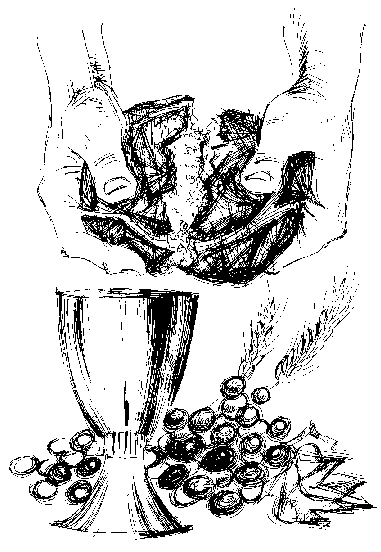
\includegraphics[scale=0.35]{gambar/Cat-1011.png}
\end{center}
\vfill
\noindent{\framebox{\parbox{10cm}{\centering\emph{
”Ya Allahku, Tritunggal yang kusembah ...\\
berilah damai di dalam jiwaku;\\
jadikanlah ini surga-Mu, tempat tinggal-Mu yang tercinta\\
dan tempat istirahat-Mu.\\
Semoga aku tak pernah meninggalkan-Mu,\\
tetapi tetap tinggal di situ, seluruhnya dan seutuhnya,\\
siap sedia di dalam imanku, sepenuhnya memuja-Mu,\\
dan sepenuhnya menyerahkan diriku kepada tindakan kreatif-Mu”}\\
(Elizabet dari Tritunggal)
}}}

\chap{Senyum Sejenak}

\setlength{\parindent}{0cm}
\section*{Bercanda}
\begin{itemize}
\item[Cewek:] Mulai hari ini kita putus!
\item[Cowok:] Kok begitu... (kaget), padahal besok aku mau belikan kamu HP yang mahal.
\item[Cewek:] Hm... (mikir-mikir), aku hanya bercanda kok, Sayang.
\item[Cowok:] Oh, sama. Aku juga bercanda.
\end{itemize}

\kutipan{"Tak bergunalah dan jahatlah orang yang hidup dengan mulut serong."\\
(Amsal 6:12)
}

\section*{Menanyai seorang angkatan laut muda}

Seorang kapten kapal laut memberi beberapa pertanyaan kepada seorang 
angkatan laut muda. \\
"Apa yang kamu lakukan jika tiba-tiba ada badai?"\\
"Aku akan melemparkan jangkar, Pak."\\
"Apa yang kamu lakukan jika ada badai datang lagi?"

"Aku akan melempar jangkar lain, Pak."

"Nah, terus bagaimana jika ada badai ketiga yang menyerang?"

"Aku akan melemparkan jangkar lain, Kapten."

"Tunggu dulu, Nak. Dari mana kamu dapat jangkar sebanyak itu?"

"Dari tempat yang sama di mana Anda mendapatkan semua badai itu, Pak."

\kutipan{"Karena sebagaimana mimpi disebabkan oleh banyak kesibukan, demikian 
pula percakapan bodoh disebabkan oleh banyak perkataan." \\
(Pengkhotbah 5:3)}
\setlength{\parindent}{1cm}
\normalsize
\chap{Warta Lingkungan}

\subsection*{APP}
Bulan Maret 2012 sudah masuk dalam masa Prapaskah. Sesuai dengan tradisi, setiap masa Prapaskah diadakan Aksi Puasa Pembangunan yang kegiatannya antara lain adalah ibadat APP di lingkungan. Untuk tahun ini Keuskupan Agung Semarang (KAS) menetapkan tema APP: \textit{Umat Katolik Sejati Harus Peduli dan Berbagi}. Dalam pelaksanaan di lingkungan St. Petrus, ibadat APP banyak diisi dengan \textit{sharing} yang mengacu pada buku panduan dari KAS.
Topik APP berawal dari baptis. Kapan kita dibaptis, kesan-kesan saat dibaptis, dan relevansinya dengan hidup menggereja dan bermasyarakat.

\subsection*{Misa pemberkatan rumah dan mitoni}
Bulan ini umat St. Petrus bertambah lagi dengan satu keluarga yang secara resmi bergabung sebagai warga lingkungan. Keluarga Bapak R. Mulyadi yang bertempat tinggal di Nanggulan, mengadakan misa syukur pemberkatan rumah dan sekaligus mitoni pada tanggal 22 Maret. Cicilia Nony Prayoga yang merupakan putri dari Bapak/Ibu Mulyadi menantikan kelahiran putranya bersama dengan suami tercinta
Bernadus Budhiprayoga.

Misa dipimpin oleh Rm. Albertus Purnomo, OFM yang merupakan kenalan baik keluarga R. Mulyadi saat masih di Jakarta. Dalam homilinya Romo menekankan bahwa Musa dapat melakukan tawar-menawar dengan Tuhan karena kedekatan Musa dengan Tuhan. Kenapa Musa dekat dengan Tuhan, karena Musa sering berdoa dan menaati perintah-Nya. Oleh karena itu kalau kita ingin dekat dengan Tuhan, maka rajin-rajinlah berdoa dan senantiasa menaati perintah-Nya.

\subsection*{Pendaftaran Krisma}
Telah diumumkan di gereja bahwa sakramen Krisma untuk paroki Marganingsih Kalasan akan dilangsungkan bulan September 2012. Calon penerima sakramen Krisma dapat mendaftarkan diri ke Ibu Munarti, Bapak Neo Suradi, atau kepada ketua lingkungan, dengan menyerahkan fotokopi surat baptis.

% SELECT day(`TglLahir`),
% concat(u1.`Baptis`,' ',u1.`Nama`) 
% FROM `umat` u1 WHERE month(TglLahir)=6 order by 1

%=========
% SELECT day(`TglNikah`),
% concat(u1.`Baptis`,' ',u1.`Nama`,' + ',u2.`Baptis`,' ',u2.`Nama`) 
% FROM `umat` u1 join kk on (u1.nokk=kk.id and u1.hubkel='KK')
%               join umat u2 on (u2.nokk=kk.id  and (u2.hubkel='istri' or u2.hubkel='isteri'))
% WHERE month(TglNikah)=1 order by 1

\section*{Yang berulang tahun kelahiran bulan ini}

\noindent{Semoga hari bahagia ini menguatkan imannya akan Dikau.}

\begin{longtable}{|c|l|} 
\hline
Tgl & Nama \\ \hline
\endhead1& Maria Rosary Sekar Seruni\\
5& Anna Maria Tri Henaningsih\\
6& Fransiscus Xaverius Sularto\\
7& Christina Sutarni\\
8& Marcellina Oktavia S. Padmini\\
11& Priscilla Oktiva Rossari\\
15& Yoseph Laba Atawolo\\
16& Ignatius Stanley Andi Pradana\\
18& Christina Sri Ning Hastuti\\
24& Margareta Maria Sri Pramuwati\\
25& Kristina Tri Tutwuri\\
\hline
\end{longtable}



\section*{Yang berulang tahun perkawinan  bulan ini}

Selamat ulang tahun perkawinan. Semoga keluarga-keluarga ini tumbuh menjadi keluarga Katolik yang sejati yang dibangun atas dasar iman dan kasih: kasih akan Dikau dan kasih antar semua anggota keluarga.

\begin{longtable}{|c|l|} 
\hline
Tgl & Keluarga \\ \hline
\endhead5& Nikolas Putut Andoko + Chatarina Krisyanti\\
6& Ignatius Luddy Indra Purnama + Anna Sri Wuryaningtyas\\
\hline
\end{longtable} 

\newpage
\chap{Kompendium Katekese Gereja Katolik}
\setcounter{kgkcounter}{37}
\normalsize
\kgk{Dengan nama apa Allah mewahyukan Diri-Nya?}
Allah mewahyukan Diri-Nya kepada Musa sebagai Allah yang hidup, ”Allah
Abraham, Allah Iskak, Allah Yakub” (Kel 3:6). Allah juga mewahyukan kepada Musa
nama-Nya yang gaib ”Aku adalah Aku (YHWH)”. Sudah sejak zaman Perjanjian
Lama, Nama Allah yang tak terkatakan ini diganti dengan gelar ilahi Tuhan. Jadi, manakala Yesus disebut Tuhan di dalam Perjanjian Baru, Ia tampil sebagai benar-benar Allah.

\kgk{Apa Allah itu satu-satunya yang ”ada”?}
Karena makhluk menerima segalanya dari Allah, mereka ada dan kepunyaan
mereka dari Allah. Hanya Allah dalam Diri-Nya sendiri merupakan kepenuhan dari
yang ada dan dari setiap kesempurnaan. Allah itu ”Dia yang ada” tanpa awal dan
tanpa akhir. Yesus mewahyukan bahwa Ia juga menyandang nama ilahi ”Aku ada”
 (Yoh 8:28).

\small

\kgk{Mengapa pewahyuan Nama Allah itu penting?}
Dalam mewahyukan nama-Nya, Allah memberitahukan kekayaan yang
 ada di dalam misteri ada-Nya yang tak terkatakan. Hanya Dia sendirilah yang
 dari kekal sampai kekal. Dia mengatasi dunia dan sejarah. Dialah yang membuat
 langit dan bumi. Dia adalah Allah yang setia yang selalu dekat dengan umat-Nya
 untuk menyelamatkan mereka. Dialah kekudusan tertinggi, ”penuh dengan belas
 kasihan” (Ef 2:4), selalu siap untuk mengampuni. Dialah yang spiritual, transenden,
 mahakuasa, personal, dan sempurna. Dia adalah kebenaran dan cinta.

\section*{Seksi Dua: Pengakuan Iman Kristen}

\kgk{Apa artinya bahwa Allah adalah Kebenaran?}
 Allah adalah Kebenaran, dengan demikian Dia tidak dapat menipu ataupun 
ditipu. Dia adalah ”terang, dan di dalam-Nya tidak ada kegelapan” (1Yoh 1:5). Putra 
Allah yang kekal, penjelmaan kebijaksanaan, diutus ke dunia untuk ”memberikan
kesaksian akan Kebenaran” (Yoh 18:37).

\flushright{(\dots \emph{bersambung} \dots)}
\normalsize
\end{document}